\chapter{METODOLOGI}
\label{chap:metodologi}

% Ubah bagian-bagian berikut dengan isi dari desain dan implementasi

Eksperimen pada penelitian ini akan mengikuti konvensi standar eksperimen DRL sebelumnya, yaitu menguji coba dan mengevaluasi performa agen dalam \emph{environment} dengan membandingkan nilai \emph{reward} yang diterima oleh agen.
Agen akan melakukan \emph{training} dalam \emph{environment} yang telah dibuat.

\section{Perangkat}
\label{sec:perangkat}

Eksperimen dalam penelitian ini menggunakan beberapa perangkat keras dan perangkat lunak.


\subsection{Perangkat Keras}
\label{subsec:perangkatkeras}

Proses \emph{training} agen dilakukan dengan sebuah komputer. Komputer tersebut memiliki spesifikasi:
\begin{itemize}
  \item Processor: Intel I7 9700K
  \item Graphics Card: RTX 2080 SUPER
  \item RAM: 32GB DDR4
  \item SSD: 512GB NVME PCIE Gen 3
\end{itemize}

\subsection{Perangkat Lunak}
\label{subsec:perangkatlunak}

Beberapa pernagkat lunak digunakan untuk menunjang pembuatan \emph{environment} dan agen DRL dalam eksperimen ini:
\begin{itemize}
  \item Python
  \item Visual Studio Code
  \item Tensorboard
  \item Ray RLlib
  \item Pygame
  \item PettingZoo
  \item Numpy
  \item Matplotlib
\end{itemize}
\section{Desain Environment}
\label{sec:desainenvironment}

Desain dari \emph{environment} adalah modifikasi dari Inquisitive Otter's Civ6 environment \citep{civ6Environment}. 
Desain awal dari \emph{environment} ini hanya memiliki sebuah agen \emph{attacker} dan memiliki mekanisme yang kurang sesuai dengan mekanisme Civ6.
\emph{Environment} merupakan area \emph{pointy top hexagonal grid} berukuran 8x8. Di tengah area tersebut terdapat sebuah \emph{city}.
\emph{Environment} yang sudah termodifikasi memiliki dua jenis agen yaitu agen \emph{attacker} dan agen \emph{defender}.
Agen \emph{attacker} memiliki 3 \emph{unit} jarak dekat (\emph{warrior}) dan 2 \emph{unit} jarak jauh (\emph{slinger}).
Agen \emph{defender} memiliki 2 \emph{warrior} dan 1 \emph{slinger}.
Penempatan \emph{unit} agen dilakukan secara acak dengan pembatasan.
\emph{Unit} agen \emph{attacker} ditempatkan minimal sejauh 5 lantai dari \emph{city} di tengah area.
\emph{Unit} agen \emph{defender} berada di lantai sebelah \emph{city}.


\begin{figure}[H]
  \centering
    % Nama dari file gambar yang diinputkan
    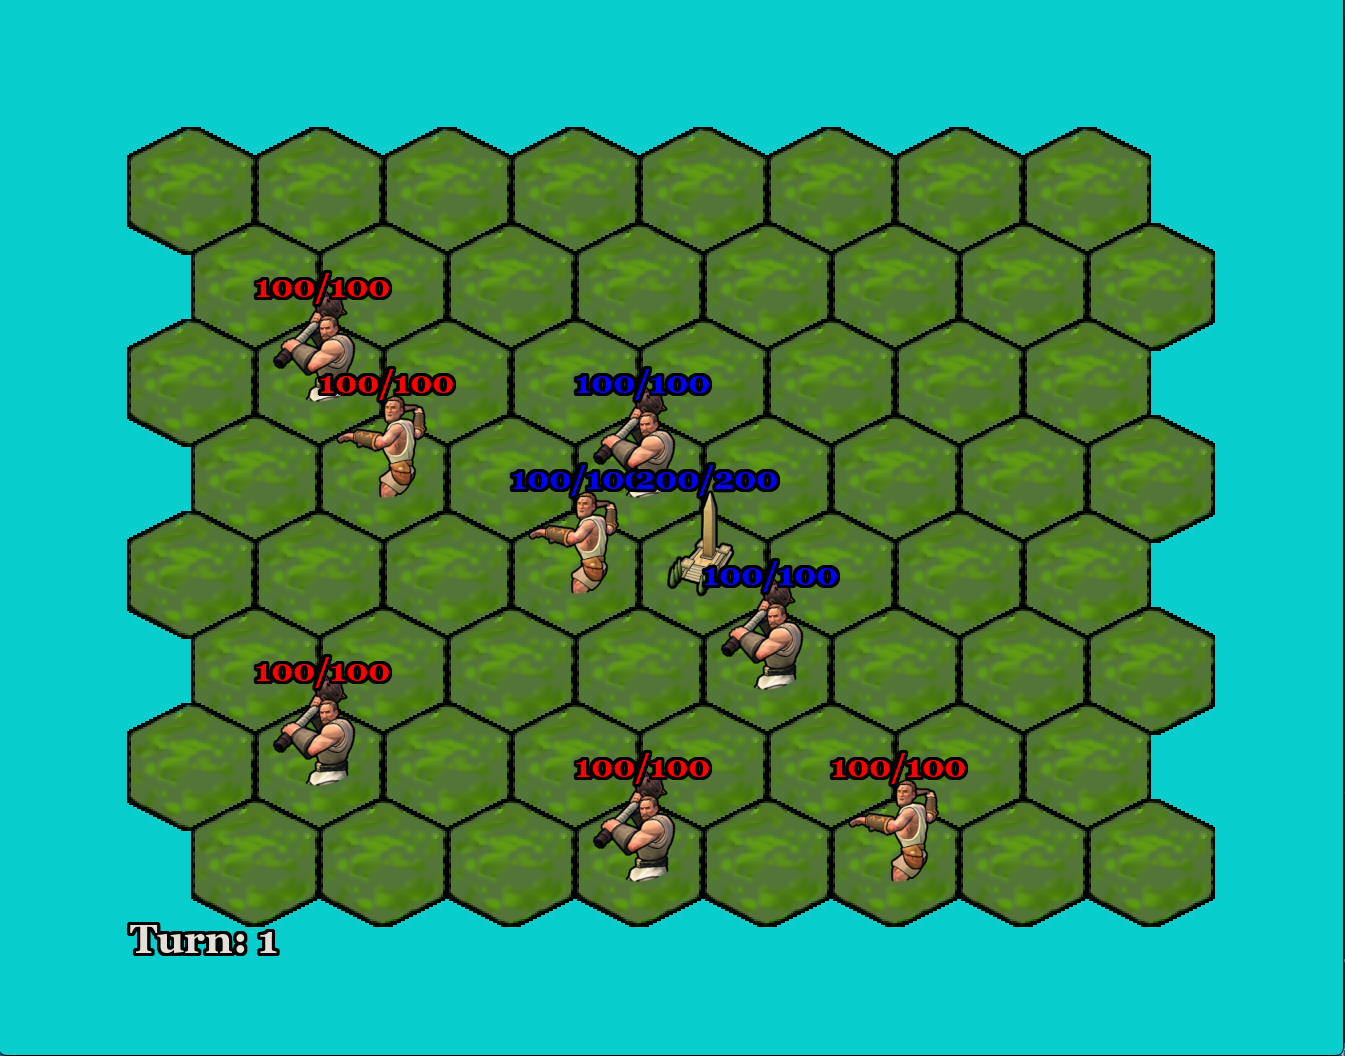
\includegraphics[scale=0.3]{gambar/environment_screenshot.png}
    % Keterangan gambar yang diinputkan
    \caption{\emph{Screenshot environment} dalam mode \emph{render}. \emph{Unit} milik agen \emph{attacker} memiliki teks \emph{hit points} berwarna merah dan unit milik agen \emph{defender} memiliki teks \emph{hit points} berwarna biru.}
    % Label referensi dari gambar yang diinputkan
    \label{fig:environmentScreenshot}
\end{figure}



% % Per blok diagram dijelaskan dan dibuatkan section masing-masing

% % \section{Blok Diagram}
% % \label{sec:blokdiagram}

% % Contoh pembuatan potongan kode
% \begin{lstlisting}[
%   language=C++,
%   caption={Program halo dunia.},
%   label={lst:halodunia}
% ]
% #include <iostream>

% int main() {
%     std::cout << "Halo Dunia!";
%     return 0;
% }
% \end{lstlisting}

% \lipsum[2-3]

% % Contoh input potongan kode dari file
% \lstinputlisting[
%   language=Python,
%   caption={Program perhitungan bilangan prima.},
%   label={lst:bilanganprima}
% ]{program/bilangan-prima.py}

% \lipsum[4]
